% Options for packages loaded elsewhere
\PassOptionsToPackage{unicode}{hyperref}
\PassOptionsToPackage{hyphens}{url}
%
\documentclass[
]{article}
\usepackage{amsmath,amssymb}
\usepackage{iftex}
\ifPDFTeX
  \usepackage[T1]{fontenc}
  \usepackage[utf8]{inputenc}
  \usepackage{textcomp} % provide euro and other symbols
\else % if luatex or xetex
  \usepackage{unicode-math} % this also loads fontspec
  \defaultfontfeatures{Scale=MatchLowercase}
  \defaultfontfeatures[\rmfamily]{Ligatures=TeX,Scale=1}
\fi
\usepackage{lmodern}
\ifPDFTeX\else
  % xetex/luatex font selection
\fi
% Use upquote if available, for straight quotes in verbatim environments
\IfFileExists{upquote.sty}{\usepackage{upquote}}{}
\IfFileExists{microtype.sty}{% use microtype if available
  \usepackage[]{microtype}
  \UseMicrotypeSet[protrusion]{basicmath} % disable protrusion for tt fonts
}{}
\makeatletter
\@ifundefined{KOMAClassName}{% if non-KOMA class
  \IfFileExists{parskip.sty}{%
    \usepackage{parskip}
  }{% else
    \setlength{\parindent}{0pt}
    \setlength{\parskip}{6pt plus 2pt minus 1pt}}
}{% if KOMA class
  \KOMAoptions{parskip=half}}
\makeatother
\usepackage{xcolor}
\usepackage[margin=1in]{geometry}
\usepackage{color}
\usepackage{fancyvrb}
\newcommand{\VerbBar}{|}
\newcommand{\VERB}{\Verb[commandchars=\\\{\}]}
\DefineVerbatimEnvironment{Highlighting}{Verbatim}{commandchars=\\\{\}}
% Add ',fontsize=\small' for more characters per line
\usepackage{framed}
\definecolor{shadecolor}{RGB}{248,248,248}
\newenvironment{Shaded}{\begin{snugshade}}{\end{snugshade}}
\newcommand{\AlertTok}[1]{\textcolor[rgb]{0.94,0.16,0.16}{#1}}
\newcommand{\AnnotationTok}[1]{\textcolor[rgb]{0.56,0.35,0.01}{\textbf{\textit{#1}}}}
\newcommand{\AttributeTok}[1]{\textcolor[rgb]{0.13,0.29,0.53}{#1}}
\newcommand{\BaseNTok}[1]{\textcolor[rgb]{0.00,0.00,0.81}{#1}}
\newcommand{\BuiltInTok}[1]{#1}
\newcommand{\CharTok}[1]{\textcolor[rgb]{0.31,0.60,0.02}{#1}}
\newcommand{\CommentTok}[1]{\textcolor[rgb]{0.56,0.35,0.01}{\textit{#1}}}
\newcommand{\CommentVarTok}[1]{\textcolor[rgb]{0.56,0.35,0.01}{\textbf{\textit{#1}}}}
\newcommand{\ConstantTok}[1]{\textcolor[rgb]{0.56,0.35,0.01}{#1}}
\newcommand{\ControlFlowTok}[1]{\textcolor[rgb]{0.13,0.29,0.53}{\textbf{#1}}}
\newcommand{\DataTypeTok}[1]{\textcolor[rgb]{0.13,0.29,0.53}{#1}}
\newcommand{\DecValTok}[1]{\textcolor[rgb]{0.00,0.00,0.81}{#1}}
\newcommand{\DocumentationTok}[1]{\textcolor[rgb]{0.56,0.35,0.01}{\textbf{\textit{#1}}}}
\newcommand{\ErrorTok}[1]{\textcolor[rgb]{0.64,0.00,0.00}{\textbf{#1}}}
\newcommand{\ExtensionTok}[1]{#1}
\newcommand{\FloatTok}[1]{\textcolor[rgb]{0.00,0.00,0.81}{#1}}
\newcommand{\FunctionTok}[1]{\textcolor[rgb]{0.13,0.29,0.53}{\textbf{#1}}}
\newcommand{\ImportTok}[1]{#1}
\newcommand{\InformationTok}[1]{\textcolor[rgb]{0.56,0.35,0.01}{\textbf{\textit{#1}}}}
\newcommand{\KeywordTok}[1]{\textcolor[rgb]{0.13,0.29,0.53}{\textbf{#1}}}
\newcommand{\NormalTok}[1]{#1}
\newcommand{\OperatorTok}[1]{\textcolor[rgb]{0.81,0.36,0.00}{\textbf{#1}}}
\newcommand{\OtherTok}[1]{\textcolor[rgb]{0.56,0.35,0.01}{#1}}
\newcommand{\PreprocessorTok}[1]{\textcolor[rgb]{0.56,0.35,0.01}{\textit{#1}}}
\newcommand{\RegionMarkerTok}[1]{#1}
\newcommand{\SpecialCharTok}[1]{\textcolor[rgb]{0.81,0.36,0.00}{\textbf{#1}}}
\newcommand{\SpecialStringTok}[1]{\textcolor[rgb]{0.31,0.60,0.02}{#1}}
\newcommand{\StringTok}[1]{\textcolor[rgb]{0.31,0.60,0.02}{#1}}
\newcommand{\VariableTok}[1]{\textcolor[rgb]{0.00,0.00,0.00}{#1}}
\newcommand{\VerbatimStringTok}[1]{\textcolor[rgb]{0.31,0.60,0.02}{#1}}
\newcommand{\WarningTok}[1]{\textcolor[rgb]{0.56,0.35,0.01}{\textbf{\textit{#1}}}}
\usepackage{graphicx}
\makeatletter
\def\maxwidth{\ifdim\Gin@nat@width>\linewidth\linewidth\else\Gin@nat@width\fi}
\def\maxheight{\ifdim\Gin@nat@height>\textheight\textheight\else\Gin@nat@height\fi}
\makeatother
% Scale images if necessary, so that they will not overflow the page
% margins by default, and it is still possible to overwrite the defaults
% using explicit options in \includegraphics[width, height, ...]{}
\setkeys{Gin}{width=\maxwidth,height=\maxheight,keepaspectratio}
% Set default figure placement to htbp
\makeatletter
\def\fps@figure{htbp}
\makeatother
\setlength{\emergencystretch}{3em} % prevent overfull lines
\providecommand{\tightlist}{%
  \setlength{\itemsep}{0pt}\setlength{\parskip}{0pt}}
\setcounter{secnumdepth}{-\maxdimen} % remove section numbering
\ifLuaTeX
  \usepackage{selnolig}  % disable illegal ligatures
\fi
\usepackage{bookmark}
\IfFileExists{xurl.sty}{\usepackage{xurl}}{} % add URL line breaks if available
\urlstyle{same}
\hypersetup{
  pdftitle={Group Project 1},
  hidelinks,
  pdfcreator={LaTeX via pandoc}}

\title{Group Project 1}
\usepackage{etoolbox}
\makeatletter
\providecommand{\subtitle}[1]{% add subtitle to \maketitle
  \apptocmd{\@title}{\par {\large #1 \par}}{}{}
}
\makeatother
\subtitle{Biology 368/664 Bucknell University}
\author{}
\date{\vspace{-2.5em}14 Sep 2024}

\begin{document}
\maketitle

\begin{Shaded}
\begin{Highlighting}[]
\CommentTok{\#Reading in the built in dataset from R}
\NormalTok{(esoph)}
\end{Highlighting}
\end{Shaded}

\begin{verbatim}
##    agegp     alcgp    tobgp ncases ncontrols
## 1  25-34 0-39g/day 0-9g/day      0        40
## 2  25-34 0-39g/day    10-19      0        10
## 3  25-34 0-39g/day    20-29      0         6
## 4  25-34 0-39g/day      30+      0         5
## 5  25-34     40-79 0-9g/day      0        27
## 6  25-34     40-79    10-19      0         7
## 7  25-34     40-79    20-29      0         4
## 8  25-34     40-79      30+      0         7
## 9  25-34    80-119 0-9g/day      0         2
## 10 25-34    80-119    10-19      0         1
## 11 25-34    80-119      30+      0         2
## 12 25-34      120+ 0-9g/day      0         1
## 13 25-34      120+    10-19      1         0
## 14 25-34      120+    20-29      0         1
## 15 25-34      120+      30+      0         2
## 16 35-44 0-39g/day 0-9g/day      0        60
## 17 35-44 0-39g/day    10-19      1        13
## 18 35-44 0-39g/day    20-29      0         7
## 19 35-44 0-39g/day      30+      0         8
## 20 35-44     40-79 0-9g/day      0        35
## 21 35-44     40-79    10-19      3        20
## 22 35-44     40-79    20-29      1        13
## 23 35-44     40-79      30+      0         8
## 24 35-44    80-119 0-9g/day      0        11
## 25 35-44    80-119    10-19      0         6
## 26 35-44    80-119    20-29      0         2
## 27 35-44    80-119      30+      0         1
## 28 35-44      120+ 0-9g/day      2         1
## 29 35-44      120+    10-19      0         3
## 30 35-44      120+    20-29      2         2
## 31 45-54 0-39g/day 0-9g/day      1        45
## 32 45-54 0-39g/day    10-19      0        18
## 33 45-54 0-39g/day    20-29      0        10
## 34 45-54 0-39g/day      30+      0         4
## 35 45-54     40-79 0-9g/day      6        32
## 36 45-54     40-79    10-19      4        17
## 37 45-54     40-79    20-29      5        10
## 38 45-54     40-79      30+      5         2
## 39 45-54    80-119 0-9g/day      3        13
## 40 45-54    80-119    10-19      6         8
## 41 45-54    80-119    20-29      1         4
## 42 45-54    80-119      30+      2         2
## 43 45-54      120+ 0-9g/day      4         0
## 44 45-54      120+    10-19      3         1
## 45 45-54      120+    20-29      2         1
## 46 45-54      120+      30+      4         0
## 47 55-64 0-39g/day 0-9g/day      2        47
## 48 55-64 0-39g/day    10-19      3        19
## 49 55-64 0-39g/day    20-29      3         9
## 50 55-64 0-39g/day      30+      4         2
## 51 55-64     40-79 0-9g/day      9        31
## 52 55-64     40-79    10-19      6        15
## 53 55-64     40-79    20-29      4        13
## 54 55-64     40-79      30+      3         3
## 55 55-64    80-119 0-9g/day      9         9
## 56 55-64    80-119    10-19      8         7
## 57 55-64    80-119    20-29      3         3
## 58 55-64    80-119      30+      4         0
## 59 55-64      120+ 0-9g/day      5         5
## 60 55-64      120+    10-19      6         1
## 61 55-64      120+    20-29      2         1
## 62 55-64      120+      30+      5         1
## 63 65-74 0-39g/day 0-9g/day      5        43
## 64 65-74 0-39g/day    10-19      4        10
## 65 65-74 0-39g/day    20-29      2         5
## 66 65-74 0-39g/day      30+      0         2
## 67 65-74     40-79 0-9g/day     17        17
## 68 65-74     40-79    10-19      3         7
## 69 65-74     40-79    20-29      5         4
## 70 65-74    80-119 0-9g/day      6         7
## 71 65-74    80-119    10-19      4         8
## 72 65-74    80-119    20-29      2         1
## 73 65-74    80-119      30+      1         0
## 74 65-74      120+ 0-9g/day      3         1
## 75 65-74      120+    10-19      1         1
## 76 65-74      120+    20-29      1         0
## 77 65-74      120+      30+      1         0
## 78   75+ 0-39g/day 0-9g/day      1        17
## 79   75+ 0-39g/day    10-19      2         4
## 80   75+ 0-39g/day      30+      1         2
## 81   75+     40-79 0-9g/day      2         3
## 82   75+     40-79    10-19      1         2
## 83   75+     40-79    20-29      0         3
## 84   75+     40-79      30+      1         0
## 85   75+    80-119 0-9g/day      1         0
## 86   75+    80-119    10-19      1         0
## 87   75+      120+ 0-9g/day      2         0
## 88   75+      120+    10-19      1         0
\end{verbatim}

\begin{Shaded}
\begin{Highlighting}[]
\FunctionTok{write.csv}\NormalTok{(esoph, }\StringTok{"Esoph.scancer.csv"}\NormalTok{, }\AttributeTok{row.names =} \ConstantTok{FALSE}\NormalTok{)}
\NormalTok{Esoph\_scancer }\OtherTok{\textless{}{-}} \FunctionTok{read.csv}\NormalTok{(}\StringTok{"Esoph.scancer.csv"}\NormalTok{)}
\end{Highlighting}
\end{Shaded}

\begin{Shaded}
\begin{Highlighting}[]
\CommentTok{\#Converting to factors}
\NormalTok{Esoph\_scancer}\SpecialCharTok{$}\NormalTok{agegp}\OtherTok{\textless{}{-}} \FunctionTok{as.factor}\NormalTok{(Esoph\_scancer}\SpecialCharTok{$}\NormalTok{agegp)}
\NormalTok{Esoph\_scancer}\SpecialCharTok{$}\NormalTok{alcgp}\OtherTok{\textless{}{-}} \FunctionTok{as.factor}\NormalTok{(Esoph\_scancer}\SpecialCharTok{$}\NormalTok{alcgp)}
\NormalTok{Esoph\_scancer}\SpecialCharTok{$}\NormalTok{tobgp}\OtherTok{\textless{}{-}} \FunctionTok{as.factor}\NormalTok{(Esoph\_scancer}\SpecialCharTok{$}\NormalTok{tobgp)}
\end{Highlighting}
\end{Shaded}

Preliminary hypothesis testing: \#\#\#Creating a hypothesis: When
creating a hypothesis, it is important to not look at the results first
as this could lead to ``harking'' or formulating a ``hypothesis after
the results are known.'' When first looking at our dataset (``esoph''
from the built-in R datasets, holds data for the age of subjects,
alcohol intake, tobacco intake, number of esophageal cancer cases, and
number of controls), we looked at the variables without checking for
normality of the data or graphing/testing our results. There were three
variables that stood out to us: alcohol intake, tobacco intake, and
number of esophageal cancer cases. This led us to formulating the
following hypothesis:

Groups that smoke/drink more may have a higher risk of developing
cancer. The number of cases may also increase with age.

Variables: Tobacco per day (g) - ordinal, categorical Alcohol per day
(g) - ordinal, categorical Age (grouped into ranges of age) - ordinal,
categorical Number of cases (numerical values that can be counted) -
discrete, quantitative

As a first look for comparisons, we can calculate the mean of each of
the groups individually to determine which groups had the highest number
of cases. This can be done using the following function:

\begin{Shaded}
\begin{Highlighting}[]
\CommentTok{\#Finding the mean number of cases for each individual group without looking into other variables}
\NormalTok{mean\_age\_group }\OtherTok{\textless{}{-}}\NormalTok{ Esoph\_scancer }\SpecialCharTok{|\textgreater{}} 
  \FunctionTok{group\_by}\NormalTok{(agegp) }\SpecialCharTok{|\textgreater{}} 
  \FunctionTok{summarize}\NormalTok{(}\AttributeTok{mean\_value =} \FunctionTok{mean}\NormalTok{(ncases, }\AttributeTok{na.rm =} \ConstantTok{TRUE}\NormalTok{))}
\NormalTok{mean\_age\_group}
\end{Highlighting}
\end{Shaded}

\begin{verbatim}
## # A tibble: 6 x 2
##   agegp mean_value
##   <fct>      <dbl>
## 1 25-34     0.0667
## 2 35-44     0.6   
## 3 45-54     2.88  
## 4 55-64     4.75  
## 5 65-74     3.67  
## 6 75+       1.18
\end{verbatim}

\begin{Shaded}
\begin{Highlighting}[]
\NormalTok{mean\_alc\_group }\OtherTok{\textless{}{-}}\NormalTok{ Esoph\_scancer }\SpecialCharTok{|\textgreater{}} 
  \FunctionTok{group\_by}\NormalTok{(alcgp) }\SpecialCharTok{|\textgreater{}} 
  \FunctionTok{summarize}\NormalTok{(}\AttributeTok{mean\_value =} \FunctionTok{mean}\NormalTok{(ncases, }\AttributeTok{na.rm =} \ConstantTok{TRUE}\NormalTok{))}
\NormalTok{mean\_alc\_group}
\end{Highlighting}
\end{Shaded}

\begin{verbatim}
## # A tibble: 4 x 2
##   alcgp     mean_value
##   <fct>          <dbl>
## 1 0-39g/day       1.26
## 2 120+            2.14
## 3 40-79           3.26
## 4 80-119          2.43
\end{verbatim}

\begin{Shaded}
\begin{Highlighting}[]
\NormalTok{mean\_tob\_group }\OtherTok{\textless{}{-}}\NormalTok{ Esoph\_scancer }\SpecialCharTok{|\textgreater{}} 
  \FunctionTok{group\_by}\NormalTok{(tobgp) }\SpecialCharTok{|\textgreater{}} 
  \FunctionTok{summarize}\NormalTok{(}\AttributeTok{mean\_value =} \FunctionTok{mean}\NormalTok{(ncases, }\AttributeTok{na.rm =} \ConstantTok{TRUE}\NormalTok{))}
\NormalTok{mean\_tob\_group}
\end{Highlighting}
\end{Shaded}

\begin{verbatim}
## # A tibble: 4 x 2
##   tobgp    mean_value
##   <fct>         <dbl>
## 1 0-9g/day       3.25
## 2 10-19          2.42
## 3 20-29          1.65
## 4 30+            1.55
\end{verbatim}

The following can be done to order the ranking by number of cases just
to see which groups had the highest number of cases and which groups had
the lowest number of cases. We can see the first and last ten rows in
the ordered dataset by using the ``head'' and ``tail'' functions.

\begin{Shaded}
\begin{Highlighting}[]
\NormalTok{ranking }\OtherTok{\textless{}{-}}\NormalTok{ Esoph\_scancer }\SpecialCharTok{|\textgreater{}}
  \FunctionTok{arrange}\NormalTok{(}\FunctionTok{desc}\NormalTok{(ncases), }\AttributeTok{.by\_group =} \ConstantTok{TRUE}\NormalTok{) }
\NormalTok{ranking}
\end{Highlighting}
\end{Shaded}

\begin{verbatim}
##    agegp     alcgp    tobgp ncases ncontrols
## 1  65-74     40-79 0-9g/day     17        17
## 2  55-64     40-79 0-9g/day      9        31
## 3  55-64    80-119 0-9g/day      9         9
## 4  55-64    80-119    10-19      8         7
## 5  45-54     40-79 0-9g/day      6        32
## 6  45-54    80-119    10-19      6         8
## 7  55-64     40-79    10-19      6        15
## 8  55-64      120+    10-19      6         1
## 9  65-74    80-119 0-9g/day      6         7
## 10 45-54     40-79    20-29      5        10
## 11 45-54     40-79      30+      5         2
## 12 55-64      120+ 0-9g/day      5         5
## 13 55-64      120+      30+      5         1
## 14 65-74 0-39g/day 0-9g/day      5        43
## 15 65-74     40-79    20-29      5         4
## 16 45-54     40-79    10-19      4        17
## 17 45-54      120+ 0-9g/day      4         0
## 18 45-54      120+      30+      4         0
## 19 55-64 0-39g/day      30+      4         2
## 20 55-64     40-79    20-29      4        13
## 21 55-64    80-119      30+      4         0
## 22 65-74 0-39g/day    10-19      4        10
## 23 65-74    80-119    10-19      4         8
## 24 35-44     40-79    10-19      3        20
## 25 45-54    80-119 0-9g/day      3        13
## 26 45-54      120+    10-19      3         1
## 27 55-64 0-39g/day    10-19      3        19
## 28 55-64 0-39g/day    20-29      3         9
## 29 55-64     40-79      30+      3         3
## 30 55-64    80-119    20-29      3         3
## 31 65-74     40-79    10-19      3         7
## 32 65-74      120+ 0-9g/day      3         1
## 33 35-44      120+ 0-9g/day      2         1
## 34 35-44      120+    20-29      2         2
## 35 45-54    80-119      30+      2         2
## 36 45-54      120+    20-29      2         1
## 37 55-64 0-39g/day 0-9g/day      2        47
## 38 55-64      120+    20-29      2         1
## 39 65-74 0-39g/day    20-29      2         5
## 40 65-74    80-119    20-29      2         1
## 41   75+ 0-39g/day    10-19      2         4
## 42   75+     40-79 0-9g/day      2         3
## 43   75+      120+ 0-9g/day      2         0
## 44 25-34      120+    10-19      1         0
## 45 35-44 0-39g/day    10-19      1        13
## 46 35-44     40-79    20-29      1        13
## 47 45-54 0-39g/day 0-9g/day      1        45
## 48 45-54    80-119    20-29      1         4
## 49 65-74    80-119      30+      1         0
## 50 65-74      120+    10-19      1         1
## 51 65-74      120+    20-29      1         0
## 52 65-74      120+      30+      1         0
## 53   75+ 0-39g/day 0-9g/day      1        17
## 54   75+ 0-39g/day      30+      1         2
## 55   75+     40-79    10-19      1         2
## 56   75+     40-79      30+      1         0
## 57   75+    80-119 0-9g/day      1         0
## 58   75+    80-119    10-19      1         0
## 59   75+      120+    10-19      1         0
## 60 25-34 0-39g/day 0-9g/day      0        40
## 61 25-34 0-39g/day    10-19      0        10
## 62 25-34 0-39g/day    20-29      0         6
## 63 25-34 0-39g/day      30+      0         5
## 64 25-34     40-79 0-9g/day      0        27
## 65 25-34     40-79    10-19      0         7
## 66 25-34     40-79    20-29      0         4
## 67 25-34     40-79      30+      0         7
## 68 25-34    80-119 0-9g/day      0         2
## 69 25-34    80-119    10-19      0         1
## 70 25-34    80-119      30+      0         2
## 71 25-34      120+ 0-9g/day      0         1
## 72 25-34      120+    20-29      0         1
## 73 25-34      120+      30+      0         2
## 74 35-44 0-39g/day 0-9g/day      0        60
## 75 35-44 0-39g/day    20-29      0         7
## 76 35-44 0-39g/day      30+      0         8
## 77 35-44     40-79 0-9g/day      0        35
## 78 35-44     40-79      30+      0         8
## 79 35-44    80-119 0-9g/day      0        11
## 80 35-44    80-119    10-19      0         6
## 81 35-44    80-119    20-29      0         2
## 82 35-44    80-119      30+      0         1
## 83 35-44      120+    10-19      0         3
## 84 45-54 0-39g/day    10-19      0        18
## 85 45-54 0-39g/day    20-29      0        10
## 86 45-54 0-39g/day      30+      0         4
## 87 65-74 0-39g/day      30+      0         2
## 88   75+     40-79    20-29      0         3
\end{verbatim}

\begin{Shaded}
\begin{Highlighting}[]
\FunctionTok{head}\NormalTok{(ranking)}
\end{Highlighting}
\end{Shaded}

\begin{verbatim}
##   agegp  alcgp    tobgp ncases ncontrols
## 1 65-74  40-79 0-9g/day     17        17
## 2 55-64  40-79 0-9g/day      9        31
## 3 55-64 80-119 0-9g/day      9         9
## 4 55-64 80-119    10-19      8         7
## 5 45-54  40-79 0-9g/day      6        32
## 6 45-54 80-119    10-19      6         8
\end{verbatim}

\begin{Shaded}
\begin{Highlighting}[]
\FunctionTok{tail}\NormalTok{(ranking)}
\end{Highlighting}
\end{Shaded}

\begin{verbatim}
##    agegp     alcgp tobgp ncases ncontrols
## 83 35-44      120+ 10-19      0         3
## 84 45-54 0-39g/day 10-19      0        18
## 85 45-54 0-39g/day 20-29      0        10
## 86 45-54 0-39g/day   30+      0         4
## 87 65-74 0-39g/day   30+      0         2
## 88   75+     40-79 20-29      0         3
\end{verbatim}

The above functions and results give us a first look into each variable
or group separately, however, this doesn't take into account all of the
factors together, so the results of this would not be reliable enough to
make any conclusions.

\#\#\#Creating a linear model:

Creating a linear model is valuable for analyzing this data because it
allows us to look into each of the explanatory variables separately and
at each of the variables' interactions with the others.

\begin{Shaded}
\begin{Highlighting}[]
\NormalTok{lm1}\OtherTok{\textless{}{-}}\FunctionTok{lm}\NormalTok{(ncases }\SpecialCharTok{\textasciitilde{}}\NormalTok{ agegp }\SpecialCharTok{*}\NormalTok{ (alcgp }\SpecialCharTok{+}\NormalTok{ tobgp), }\AttributeTok{data=}\NormalTok{Esoph\_scancer) }
\FunctionTok{summary}\NormalTok{(lm1)}
\end{Highlighting}
\end{Shaded}

\begin{verbatim}
## 
## Call:
## lm(formula = ncases ~ agegp * (alcgp + tobgp), data = Esoph_scancer)
## 
## Residuals:
##     Min      1Q  Median      3Q     Max 
## -3.9167 -0.5937  0.0278  0.4375  5.3333 
## 
## Coefficients:
##                          Estimate Std. Error t value Pr(>|t|)    
## (Intercept)            -5.556e-02  1.083e+00  -0.051  0.95932    
## agegp35-44              1.944e-01  1.532e+00   0.127  0.89956    
## agegp45-54              9.306e-01  1.526e+00   0.610  0.54500    
## agegp55-64              4.556e+00  1.526e+00   2.985  0.00453 ** 
## agegp65-74              6.750e+00  1.532e+00   4.406 6.25e-05 ***
## agegp75+                1.681e+00  1.614e+00   1.041  0.30309    
## alcgp120+               2.500e-01  1.149e+00   0.218  0.82872    
## alcgp40-79              9.216e-15  1.149e+00   0.000  1.00000    
## alcgp80-119            -2.778e-02  1.270e+00  -0.022  0.98265    
## tobgp10-19              2.500e-01  1.149e+00   0.218  0.82872    
## tobgp20-29             -2.778e-02  1.270e+00  -0.022  0.98265    
## tobgp30+               -7.542e-15  1.149e+00   0.000  1.00000    
## agegp35-44:alcgp120+    6.944e-01  1.713e+00   0.405  0.68704    
## agegp45-54:alcgp120+    2.750e+00  1.625e+00   1.692  0.09734 .  
## agegp55-64:alcgp120+    1.250e+00  1.625e+00   0.769  0.44567    
## agegp65-74:alcgp120+   -1.500e+00  1.625e+00  -0.923  0.36076    
## agegp75+:alcgp120+     -2.500e-01  1.934e+00  -0.129  0.89771    
## agegp35-44:alcgp40-79   7.500e-01  1.625e+00   0.462  0.64657    
## agegp45-54:alcgp40-79   4.750e+00  1.625e+00   2.923  0.00536 ** 
## agegp55-64:alcgp40-79   2.500e+00  1.625e+00   1.539  0.13077    
## agegp65-74:alcgp40-79   4.972e+00  1.713e+00   2.903  0.00566 ** 
## agegp75+:alcgp40-79    -8.499e-15  1.755e+00   0.000  1.00000    
## agegp35-44:alcgp80-119 -2.222e-01  1.713e+00  -0.130  0.89734    
## agegp45-54:alcgp80-119  2.778e+00  1.713e+00   1.622  0.11169    
## agegp55-64:alcgp80-119  3.028e+00  1.713e+00   1.768  0.08374 .  
## agegp65-74:alcgp80-119  5.278e-01  1.713e+00   0.308  0.75937    
## agegp75+:alcgp80-119   -4.722e-01  2.008e+00  -0.235  0.81516    
## agegp35-44:tobgp10-19   2.500e-01  1.625e+00   0.154  0.87840    
## agegp45-54:tobgp10-19  -5.000e-01  1.625e+00  -0.308  0.75970    
## agegp55-64:tobgp10-19  -7.500e-01  1.625e+00  -0.462  0.64657    
## agegp65-74:tobgp10-19  -5.000e+00  1.625e+00  -3.077  0.00352 ** 
## agegp75+:tobgp10-19    -5.000e-01  1.625e+00  -0.308  0.75970    
## agegp35-44:tobgp20-29   2.778e-01  1.713e+00   0.162  0.87188    
## agegp45-54:tobgp20-29  -1.472e+00  1.713e+00  -0.860  0.39451    
## agegp55-64:tobgp20-29  -3.222e+00  1.713e+00  -1.881  0.06628 .  
## agegp65-74:tobgp20-29  -5.222e+00  1.713e+00  -3.049  0.00380 ** 
## agegp75+:tobgp20-29    -1.597e+00  2.384e+00  -0.670  0.50625    
## agegp35-44:tobgp30+    -3.056e-01  1.713e+00  -0.178  0.85920    
## agegp45-54:tobgp30+    -7.500e-01  1.625e+00  -0.462  0.64657    
## agegp55-64:tobgp30+    -2.250e+00  1.625e+00  -1.385  0.17283    
## agegp65-74:tobgp30+    -5.778e+00  1.713e+00  -3.373  0.00152 ** 
## agegp75+:tobgp30+      -6.250e-01  1.905e+00  -0.328  0.74439    
## ---
## Signif. codes:  0 '***' 0.001 '**' 0.01 '*' 0.05 '.' 0.1 ' ' 1
## 
## Residual standard error: 1.625 on 46 degrees of freedom
## Multiple R-squared:  0.8158, Adjusted R-squared:  0.6517 
## F-statistic:  4.97 on 41 and 46 DF,  p-value: 1.908e-07
\end{verbatim}

The overall p-value for this linear model is extremely small. Smaller
p-values indicate that the relationship between variables is
statistically significant, and therefore this shows that there is a
significant relationship between each of the variables on number of
cases.

In order to use a linear model, there are a few assumptions that must be
followed relating to the residuals. These include the following: 1)
Independence of data points 2) Normally distributed residuals 3)
Homoscedastic data

The following test (the Durbin-Watson test) can be used to determine
autocorrelation (independence of data points).

\begin{Shaded}
\begin{Highlighting}[]
\FunctionTok{dwtest}\NormalTok{(lm1)}
\end{Highlighting}
\end{Shaded}

\begin{verbatim}
## 
##  Durbin-Watson test
## 
## data:  lm1
## DW = 2.5508, p-value = 0.6399
## alternative hypothesis: true autocorrelation is greater than 0
\end{verbatim}

The results of this show a high p-value of 0.6399, and this means that
we fail to reject the null hypothesis (which was that there is positive
autocorrelation in the residuals). The Durbin-Watson statistic is also
close enough to the ideal value of 2. Due to these results, we can
conclude that the data points are independent enough to proceed with a
linear model.

Creating a histogram can be done to determine if the residuals are
normally distributed.

\begin{Shaded}
\begin{Highlighting}[]
\FunctionTok{hist}\NormalTok{(lm1}\SpecialCharTok{$}\NormalTok{residuals, }
     \AttributeTok{main =} \StringTok{"Histogram of Residuals for Linear Model"}\NormalTok{,  }
     \AttributeTok{xlab =} \StringTok{"Residuals"}\NormalTok{, }
     \AttributeTok{col =} \StringTok{"gray"}\NormalTok{, }
     \AttributeTok{border =} \StringTok{"black"}\NormalTok{)}
\end{Highlighting}
\end{Shaded}

\includegraphics{Project01_files/figure-latex/unnamed-chunk-8-1.pdf}
This histogram shows that the residuals are normally distributed enough
for creating linear models.

We can determine homoscedasticity by plotting the linear model and
assessing the qqplot created.

\begin{Shaded}
\begin{Highlighting}[]
\FunctionTok{plot}\NormalTok{(lm1)}
\end{Highlighting}
\end{Shaded}

\begin{verbatim}
## Warning: not plotting observations with leverage one:
##   83
\end{verbatim}

\includegraphics{Project01_files/figure-latex/unnamed-chunk-9-1.pdf}
\includegraphics{Project01_files/figure-latex/unnamed-chunk-9-2.pdf}
\includegraphics{Project01_files/figure-latex/unnamed-chunk-9-3.pdf}
\includegraphics{Project01_files/figure-latex/unnamed-chunk-9-4.pdf}
Since the points mainly lie along the line of the qqplot, this tells us
that it is homoscedastic. Due to all of the assumptions being met, we
can consider a linear model an effective analysis.

An anova test can be conducted on the linear model to determine the
statistical significance of each group.

\begin{Shaded}
\begin{Highlighting}[]
\FunctionTok{anova}\NormalTok{(lm1)}
\end{Highlighting}
\end{Shaded}

\begin{verbatim}
## Analysis of Variance Table
## 
## Response: ncases
##             Df  Sum Sq Mean Sq F value    Pr(>F)    
## agegp        5 261.202  52.240 19.7850 1.796e-10 ***
## alcgp        3  52.695  17.565  6.6524 0.0007955 ***
## tobgp        3  54.706  18.235  6.9063 0.0006179 ***
## agegp:alcgp 15 100.158   6.677  2.5289 0.0080789 ** 
## agegp:tobgp 15  69.235   4.616  1.7481 0.0742146 .  
## Residuals   46 121.458   2.640                      
## ---
## Signif. codes:  0 '***' 0.001 '**' 0.01 '*' 0.05 '.' 0.1 ' ' 1
\end{verbatim}

This anova tests yields many results as it shows the significance of
each group (tobacco and alcohol intake). It shows that the results are
significant for all of the groups except for age group correlated with
tobacco group.

\begin{Shaded}
\begin{Highlighting}[]
\CommentTok{\#testing for normality in the data}
\FunctionTok{library}\NormalTok{(ggplot2)}
\FunctionTok{library}\NormalTok{(cowplot)}
\NormalTok{a }\OtherTok{\textless{}{-}} \FunctionTok{ggplot}\NormalTok{(Esoph\_scancer, }\FunctionTok{aes}\NormalTok{(}\AttributeTok{x=}\NormalTok{tobgp)) }\SpecialCharTok{+} \FunctionTok{geom\_bar}\NormalTok{() }\SpecialCharTok{+} \FunctionTok{ggtitle}\NormalTok{(}\StringTok{"Tobacco Group"}\NormalTok{)}
\NormalTok{b }\OtherTok{\textless{}{-}} \FunctionTok{ggplot}\NormalTok{(Esoph\_scancer, }\FunctionTok{aes}\NormalTok{(}\AttributeTok{x=}\NormalTok{alcgp)) }\SpecialCharTok{+} \FunctionTok{geom\_bar}\NormalTok{() }\SpecialCharTok{+} \FunctionTok{ggtitle}\NormalTok{(}\StringTok{"Alcohol Group"}\NormalTok{)}
\NormalTok{c }\OtherTok{\textless{}{-}} \FunctionTok{ggplot}\NormalTok{(Esoph\_scancer, }\FunctionTok{aes}\NormalTok{(}\AttributeTok{x=}\NormalTok{agegp)) }\SpecialCharTok{+} \FunctionTok{geom\_bar}\NormalTok{() }\SpecialCharTok{+} \FunctionTok{ggtitle}\NormalTok{(}\StringTok{"Age Group"}\NormalTok{)}

\CommentTok{\# Display the plots in a grid}
\FunctionTok{plot\_grid}\NormalTok{(a, b, c, }\AttributeTok{ncol =} \DecValTok{2}\NormalTok{)}
\end{Highlighting}
\end{Shaded}

\includegraphics{Project01_files/figure-latex/unnamed-chunk-11-1.pdf}

\#Making a histogram of the orginal and log transformed data and making
density plots of them

\begin{Shaded}
\begin{Highlighting}[]
\CommentTok{\# Create bar plots for discrete variables}
\NormalTok{a }\OtherTok{\textless{}{-}} \FunctionTok{ggplot}\NormalTok{(Esoph\_scancer, }\FunctionTok{aes}\NormalTok{(}\AttributeTok{x=}\NormalTok{tobgp)) }\SpecialCharTok{+} \FunctionTok{geom\_bar}\NormalTok{() }\SpecialCharTok{+} \FunctionTok{ggtitle}\NormalTok{(}\StringTok{"Tobacco Group {-} Bar Plot"}\NormalTok{)}
\NormalTok{b }\OtherTok{\textless{}{-}} \FunctionTok{ggplot}\NormalTok{(Esoph\_scancer, }\FunctionTok{aes}\NormalTok{(}\AttributeTok{x=}\NormalTok{alcgp)) }\SpecialCharTok{+} \FunctionTok{geom\_bar}\NormalTok{() }\SpecialCharTok{+} \FunctionTok{ggtitle}\NormalTok{(}\StringTok{"Alcohol Group {-} Bar Plot"}\NormalTok{)}

\CommentTok{\# Create density plots using continuous data (if needed)}
\CommentTok{\# Assuming there is a continuous variable, for example, ncases}
\CommentTok{\# If not, density plots may not be applicable to this dataset}

\CommentTok{\# For demonstration, let\textquotesingle{}s assume a continuous variable ncases exists}
\NormalTok{c }\OtherTok{\textless{}{-}} \FunctionTok{ggplot}\NormalTok{(Esoph\_scancer, }\FunctionTok{aes}\NormalTok{(}\AttributeTok{x=}\NormalTok{ncases)) }\SpecialCharTok{+} \FunctionTok{geom\_density}\NormalTok{() }\SpecialCharTok{+} \FunctionTok{ggtitle}\NormalTok{(}\StringTok{"Density Plot {-} ncases"}\NormalTok{)}
\NormalTok{d }\OtherTok{\textless{}{-}} \FunctionTok{ggplot}\NormalTok{(Esoph\_scancer, }\FunctionTok{aes}\NormalTok{(}\AttributeTok{x=}\FunctionTok{log}\NormalTok{(ncases))) }\SpecialCharTok{+} \FunctionTok{geom\_density}\NormalTok{() }\SpecialCharTok{+} \FunctionTok{ggtitle}\NormalTok{(}\StringTok{"Density Plot {-} log(ncases)"}\NormalTok{)}

\CommentTok{\# Plot in a 2x2 grid}
\FunctionTok{plot\_grid}\NormalTok{(a, b, c, d, }\AttributeTok{ncol =} \DecValTok{2}\NormalTok{, }\AttributeTok{nrow =} \DecValTok{2}\NormalTok{)}
\end{Highlighting}
\end{Shaded}

\begin{verbatim}
## Warning: Removed 29 rows containing non-finite outside the scale range
## (`stat_density()`).
\end{verbatim}

\includegraphics{Project01_files/figure-latex/unnamed-chunk-12-1.pdf}

\#\#\#Data Visualization Data visualization is another important aspect
of data analysis because it allows you to simplify the data in a way
that is easily digestible but still keep the importance of the findings.
Another important reason to visualize the data is that most times, you
will be presenting your findings to other people. There's also a good
chance that your audience isn't as familiar with looking at data like
you are so visuals are the best way to showcase your work.

Depending on the type of variables you are using, the kind of plot you
will want to use will be different. For example, if you are comparing a
quantitative variable with a categorical one, the type of visuals you
will wabt to use includes bar charts, boxplots, or pie charts. If you
are comparing a quantitative variable to another quantitative variable,
the type of graphs you will want to use includes a scatterplot or a line
graph. Finally, in rare cases(such as this one) comparing two
categorical variables you will want use a mosaic plot.

Our data set only uses categorical variables so we will be using a
mosaic plot along with some bar charts we used above.

\begin{Shaded}
\begin{Highlighting}[]
\FunctionTok{require}\NormalTok{(stats)}
\FunctionTok{require}\NormalTok{(graphics) }\CommentTok{\# for mosaicplot}
\FunctionTok{summary}\NormalTok{(esoph)}
\end{Highlighting}
\end{Shaded}

\begin{verbatim}
##    agegp          alcgp         tobgp        ncases         ncontrols     
##  25-34:15   0-39g/day:23   0-9g/day:24   Min.   : 0.000   Min.   : 0.000  
##  35-44:15   40-79    :23   10-19   :24   1st Qu.: 0.000   1st Qu.: 1.000  
##  45-54:16   80-119   :21   20-29   :20   Median : 1.000   Median : 4.000  
##  55-64:16   120+     :21   30+     :20   Mean   : 2.273   Mean   : 8.807  
##  65-74:15                                3rd Qu.: 4.000   3rd Qu.:10.000  
##  75+  :11                                Max.   :17.000   Max.   :60.000
\end{verbatim}

\begin{Shaded}
\begin{Highlighting}[]
\DocumentationTok{\#\# effects of alcohol, tobacco and interaction, age{-}adjusted}
\NormalTok{model1 }\OtherTok{\textless{}{-}} \FunctionTok{glm}\NormalTok{(}\FunctionTok{cbind}\NormalTok{(ncases, ncontrols) }\SpecialCharTok{\textasciitilde{}}\NormalTok{ agegp }\SpecialCharTok{+}\NormalTok{ tobgp }\SpecialCharTok{*}\NormalTok{ alcgp,}
              \AttributeTok{data =}\NormalTok{ esoph, }\AttributeTok{family =} \FunctionTok{binomial}\NormalTok{())}
\FunctionTok{anova}\NormalTok{(model1)}
\end{Highlighting}
\end{Shaded}

\begin{verbatim}
## Analysis of Deviance Table
## 
## Model: binomial, link: logit
## 
## Response: cbind(ncases, ncontrols)
## 
## Terms added sequentially (first to last)
## 
## 
##             Df Deviance Resid. Df Resid. Dev  Pr(>Chi)    
## NULL                           87     367.95              
## agegp        5  121.045        82     246.91 < 2.2e-16 ***
## tobgp        3   36.639        79     210.27 5.485e-08 ***
## alcgp        3  127.933        76      82.34 < 2.2e-16 ***
## tobgp:alcgp  9    5.451        67      76.89    0.7934    
## ---
## Signif. codes:  0 '***' 0.001 '**' 0.01 '*' 0.05 '.' 0.1 ' ' 1
\end{verbatim}

\begin{Shaded}
\begin{Highlighting}[]
\DocumentationTok{\#\# Try a linear effect of alcohol and tobacco}
\NormalTok{model2 }\OtherTok{\textless{}{-}} \FunctionTok{glm}\NormalTok{(}\FunctionTok{cbind}\NormalTok{(ncases, ncontrols) }\SpecialCharTok{\textasciitilde{}}\NormalTok{ agegp }\SpecialCharTok{+} \FunctionTok{unclass}\NormalTok{(tobgp)}
                                         \SpecialCharTok{+} \FunctionTok{unclass}\NormalTok{(alcgp),}
              \AttributeTok{data =}\NormalTok{ esoph, }\AttributeTok{family =} \FunctionTok{binomial}\NormalTok{())}
\FunctionTok{summary}\NormalTok{(model2)}
\end{Highlighting}
\end{Shaded}

\begin{verbatim}
## 
## Call:
## glm(formula = cbind(ncases, ncontrols) ~ agegp + unclass(tobgp) + 
##     unclass(alcgp), family = binomial(), data = esoph)
## 
## Coefficients:
##                Estimate Std. Error z value Pr(>|z|)    
## (Intercept)    -4.92067    0.37344 -13.177  < 2e-16 ***
## agegp.L         3.81892    0.67862   5.627 1.83e-08 ***
## agegp.Q        -1.49473    0.60671  -2.464   0.0138 *  
## agegp.C         0.07923    0.46318   0.171   0.8642    
## agegp^4         0.12136    0.32203   0.377   0.7063    
## agegp^5        -0.24856    0.21153  -1.175   0.2400    
## unclass(tobgp)  0.43955    0.09623   4.568 4.93e-06 ***
## unclass(alcgp)  1.06766    0.10493  10.175  < 2e-16 ***
## ---
## Signif. codes:  0 '***' 0.001 '**' 0.01 '*' 0.05 '.' 0.1 ' ' 1
## 
## (Dispersion parameter for binomial family taken to be 1)
## 
##     Null deviance: 367.953  on 87  degrees of freedom
## Residual deviance:  91.121  on 80  degrees of freedom
## AIC: 222.18
## 
## Number of Fisher Scoring iterations: 6
\end{verbatim}

\begin{Shaded}
\begin{Highlighting}[]
\DocumentationTok{\#\# Re{-}arrange data for a mosaic plot}
\NormalTok{ttt }\OtherTok{\textless{}{-}} \FunctionTok{table}\NormalTok{(esoph}\SpecialCharTok{$}\NormalTok{agegp, esoph}\SpecialCharTok{$}\NormalTok{alcgp, esoph}\SpecialCharTok{$}\NormalTok{tobgp)}
\NormalTok{o }\OtherTok{\textless{}{-}} \FunctionTok{with}\NormalTok{(esoph, }\FunctionTok{order}\NormalTok{(tobgp, alcgp, agegp))}
\NormalTok{ttt[ttt }\SpecialCharTok{==} \DecValTok{1}\NormalTok{] }\OtherTok{\textless{}{-}}\NormalTok{ esoph}\SpecialCharTok{$}\NormalTok{ncases[o]}
\NormalTok{tt1 }\OtherTok{\textless{}{-}} \FunctionTok{table}\NormalTok{(esoph}\SpecialCharTok{$}\NormalTok{agegp, esoph}\SpecialCharTok{$}\NormalTok{alcgp, esoph}\SpecialCharTok{$}\NormalTok{tobgp)}
\NormalTok{tt1[tt1 }\SpecialCharTok{==} \DecValTok{1}\NormalTok{] }\OtherTok{\textless{}{-}}\NormalTok{ esoph}\SpecialCharTok{$}\NormalTok{ncontrols[o]}
\NormalTok{tt }\OtherTok{\textless{}{-}} \FunctionTok{array}\NormalTok{(}\FunctionTok{c}\NormalTok{(ttt, tt1), }\FunctionTok{c}\NormalTok{(}\FunctionTok{dim}\NormalTok{(ttt),}\DecValTok{2}\NormalTok{),}
            \FunctionTok{c}\NormalTok{(}\FunctionTok{dimnames}\NormalTok{(ttt), }\FunctionTok{list}\NormalTok{(}\FunctionTok{c}\NormalTok{(}\StringTok{"Cancer"}\NormalTok{, }\StringTok{"control"}\NormalTok{))))}
\FunctionTok{mosaicplot}\NormalTok{(tt, }\AttributeTok{main =} \StringTok{"esoph data set"}\NormalTok{, }\AttributeTok{color =} \ConstantTok{TRUE}\NormalTok{)}
\end{Highlighting}
\end{Shaded}

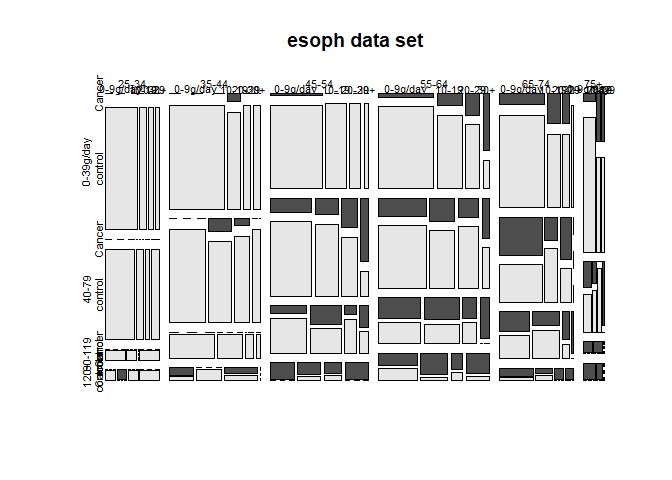
\includegraphics{Project01_files/figure-latex/- Data Visualization-1.pdf}

By making a mosaic plot we can see that there are more cancer cases in
older age groups that consume bother tobacco and alcohol compared to the
lower age group and the groups that consume either a very low amount of
each substance or none at all. The ANOVA test we performed alongside it
also tell us the signnificance of each of our groups.

\end{document}
